\documentclass[10pt,aspectratio=169]{beamer}
\usepackage{xpatch}

% ----------------------------------------------------------------
% PACKAGES & THEMES
% ----------------------------------------------------------------
\xpatchcmd{\itemize}
  {\def\makelabel}
  {\ifnum\@itemdepth=1\relax
     \setlength\itemsep{4ex}% separation for first level
   \else
     \ifnum\@itemdepth=2\relax
       \setlength\itemsep{2.5ex}% separation for second level
     \else
       \ifnum\@itemdepth=3\relax
         \setlength\itemsep{1ex}% separation for third level
   \fi\fi\fi\def\makelabel
  }
 {}
 {}
 
\usetheme{Madrid}
\usefonttheme{professionalfonts}
\usepackage{amsmath, amssymb, bm}
\usepackage{graphicx}

% ----------------------------------------------------------------
% TITLE INFORMATION
% ----------------------------------------------------------------
\title{PPO for Bipedal Walker}
\subtitle{Learning to Walk}
\author{Rushil Gupta}
\date{30th April 2025}

% ----------------------------------------------------------------
\begin{document}

\begin{frame}[plain]
  \titlepage
\end{frame}


\AtBeginSection[]
{
  \begin{frame}
    \frametitle{Table of Contents}
    \tableofcontents[currentsection]
  \end{frame}
}

% ================================================================
% SECTION 1 - INTRODUCTION
% ================================================================
\section{Introduction}

\begin{frame}{The Bipedal Walker Problem}
\begin{itemize}
  \item \textbf{Observation (state) $\bm{s}\in\mathbb{R}^{24}$}: joint angles, velocities, LIDAR-like terrain scans, hull position/velocity.
  \item \textbf{Action $\bm{a}\in[-1,1]^4$}: continuous torques for two hips and two knees.
  \item \textbf{Reward}: distance progressed $+\,$stability bonus $-\,$joint power -\,penalties; episode terminates upon fall or timeout.
\end{itemize}
\end{frame}

\begin{frame}{Two Difficulty Modes}
\begin{block}{Normal}
  Flat or mildly irregular terrain.
\end{block}
\begin{block}{Hardcore}
  Random ladders, stumps, gaps and slippery surfaces — significantly sparser rewards and higher variance.
\end{block}
\begin{figure}[h]
  \centering
  \begin{minipage}{0.375\textwidth}
    \centering
    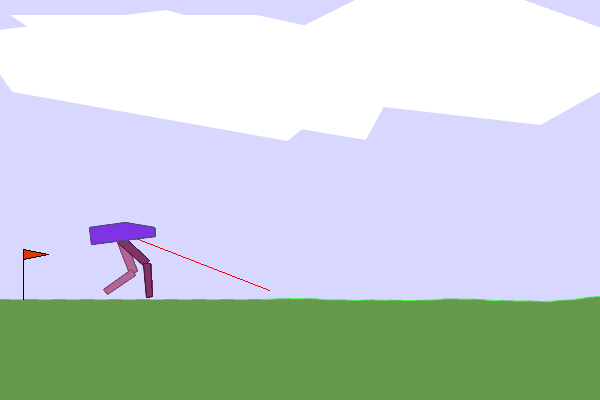
\includegraphics[width=\textwidth]{normal_mode_placeholder.png}
  \end{minipage}\hspace{0.05\textwidth}%
  \begin{minipage}{0.375\textwidth}
    \centering
    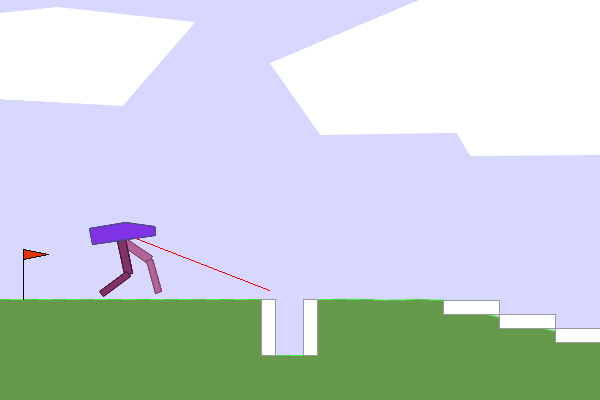
\includegraphics[width=\textwidth]{hardcore_mode_placeholder.png}
  \end{minipage}
  \caption{Environment visuals.}
\end{figure}
\end{frame}

% ================================================================
% SECTION 2 - METHODOLOGY
% ================================================================
\section{Methodology: Proximal Policy Optimization}

\begin{frame}{Implementation Overview}
\begin{itemize}
  \item We will use PPO to learn the policy
  \item Our implementation consists of two key networks:
  \begin{itemize}
    \item \textbf{Value Network}: Estimates state values $V(s)$ to compute advantages
    \begin{itemize}
      \item Implemented as an MLP with ReLU activations that outputs a scalar
      \item Used for critic updates and advantage estimation
    \end{itemize}
    \item \textbf{Gaussian Policy Network}: Produces continuous actions with exploration
    \begin{itemize}
      \item Outputs mean $\mu(s)$ and state-dependent standard deviation $\sigma(s)$
      \item Actions sampled from $\mathcal{N}(\mu(s), \sigma(s)^2)$ and squashed to $[-1, 1]$ with $\tanh$
    \end{itemize}
  \end{itemize}
\end{itemize}
\end{frame}

\begin{frame}{PPO Clipped Objective}
\small
PPO maximises the surrogate objective function:
\begin{equation*}
\mathcal{L}^{\text{clip}}(\theta) = \mathbb{E}_t\Big[\min\big(r_t(\theta)\,\hat{A}_t,\;\text{clip}\big(r_t(\theta),1-\varepsilon,1+\varepsilon\big)\,\hat{A}_t\big)\Big],
\end{equation*}
where:
\begin{itemize}
  \item $r_t(\theta)=\dfrac{\pi_\theta(\bm{a}_t|\bm{s}_t)}{\pi_{\theta_{\text{old}}}(\bm{a}_t|\bm{s}_t)}$ is the probability ratio between new and old policies
  \item $\hat{A}_t$ is the advantage estimate, computed using GAE:
\end{itemize}
\begin{align*}
\delta_t &= r_t + \gamma V_{\phi_{\text{old}}}(\bm{s}_{t+1}) - V_{\phi_{\text{old}}}(\bm{s}_{t}),\\
\hat{A}_t &= \sum_{l=0}^{T-t-1} (\gamma\lambda)^l\,\delta_{t+l}.
\end{align*}
\end{frame}

\begin{frame}{PPO Complete Loss Function}
\small
The complete loss combines three components:
\begin{equation*}
\mathcal{J}(\theta,\phi)=\mathcal{L}^{\text{clip}}-\beta\,\mathbb{E}[\mathsf{H}[\pi_\theta]]+\dfrac{c_v}{2}\,\mathbb{E}_t[(V_\phi-\hat{R}_t)^2].
\end{equation*}

\begin{itemize}
  \item $\mathcal{L}^{\text{clip}}$: Policy loss with clipping to constrain policy updates
  \item $\mathsf{H}[\pi_\theta]$: Entropy term that encourages exploration
  \begin{itemize}
    \item For Gaussian policy: $\mathsf{H}[\pi_\theta] = \frac{1}{2}\log(2\pi e \sigma^2)$
    \item Higher entropy = more exploration (wider action distribution)
    \item $\beta$ coefficient is annealed over time to reduce exploration gradually
  \end{itemize}
  \item Value loss: $\frac{c_v}{2}\,\mathbb{E}_t[(V_\phi-\hat{R}_t)^2]$ trains the critic to accurately predict returns
\end{itemize}
\end{frame}

\begin{frame}{Training Loop (GAE + Normalisation)}
\begin{itemize}
  \item \textbf{Collect} $N$ steps (or full episodes) with current policy.
  \item \textbf{Update running mean/std} $\mu,\sigma$ and normalise states: $\tilde{\bm{s}}=(\bm{s}-\mu)/\sigma$.
  \item \textbf{Compute} $\hat{A}_t$ and \emph{standardise} them: $\hat{A}\leftarrow(\hat{A}-\bar{A})/\text{Std}(\hat{A})$.
  \item \textbf{Optimise} $K$ epochs over shuffled minibatches with the clipped loss.
  \item \textbf{Anneal} entropy coefficient $\beta$ and cosine-decay learning rate.
\end{itemize}
\end{frame}

% ================================================================
% SECTION 3 - RESULTS: NORMAL MODE
% ================================================================
\section{Results I: Normal Mode}

\begin{frame}{Demonstration - Normal Mode}
\href{https://github.com/RushilGupta4/CS-5410/tree/main/Walker/gifs/normal_final.gif}{Click here}.
\end{frame}

% ================================================================
% SECTION 4 - RESULTS: HARDCORE MODE (FROM SCRATCH)
% ================================================================
\section{Results II: Hardcore Mode (From Scratch)}

\begin{frame}{Learning Challenge}
\begin{itemize}
  \item Sparse rewards and random obstacles $\Rightarrow$ frequent early terminations.
  \item The agent is not able to learn how to walk effectively, since it \textbf{falls}, or \textbf{stumbles} too often.
\end{itemize}
\end{frame}

\begin{frame}{Demonstration - Hardcore (failed)}
\href{https://github.com/RushilGupta4/CS-5410/tree/main/Walker/gifs/hardcore_fail.gif}{Click here}.
\end{frame}

% ================================================================
% SECTION 5 - RESULTS: TRANSFER LEARNING
% ================================================================
\section{Results III: Transfer Learning to Hardcore}

\begin{frame}{Warm-Start Strategy}
\begin{enumerate}
  \item \textbf{Pre-train} policy on normal terrain until convergence.\\[1.75em]
  \item \textbf{Initialise} hardcore agent with \,$\theta_{0}=\theta_{\text{normal}}$.\\[1.75em]
  \item Continue PPO fine-tuning (smaller LR, larger $\varepsilon$).
\end{enumerate}
\end{frame}

\begin{frame}{Demonstration - Hardcore (after Transfer)}
\href{https://github.com/RushilGupta4/CS-5410/tree/main/Walker/gifs/hardcore_final.gif}{Click here}.
\end{frame}

% ----------------------------------------------------------------
\end{document}
